\subsection{Game}

The Game class handles the game loop and the lifecycle of the game. To start
running a Game just call \texttt{run()} and the Game instance will enter the
following flow chart. The flow chart shows the lifecycle of a Game and the
different steps that happen through it.


\begin{figure}[H]
    \centering
    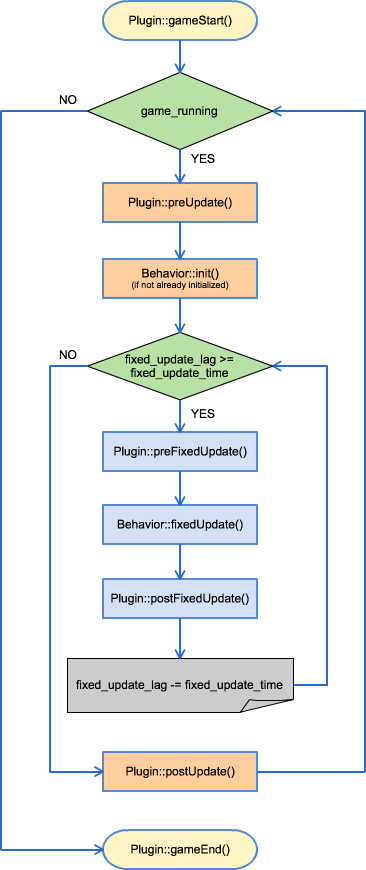
\includegraphics[width=0.5\textwidth]{game_loop}
    \caption{Game loop}
    \label{fig:game_loop}
\end{figure}

A Game instance can be queried for Time information at any step (when the
Game is running). This information can be the deltaTime(), which is the Time
that passed between the previous \texttt{update} and the current \texttt{update}; the fixedUpdateTime() which is
the Time that passes between \texttt{fixedUpdate} and \texttt{fixedUpdate} and is calculated
from the \texttt{fixed\_tickrate} constructor parameter; and the
fixedUpdateLag(), this last value is the Time since the last \texttt{fixedUpdate}.

The running state of the Game can be controlled by using setRunning(). If set
to \texttt{false} the game loop will exit and the Game will end. A Game instance
should not be reused once the Game is done running, as the final state is not
guaranteed in any way.

The Game class also owns the Actor object pool and therefore handles the
creation and destruction of Actors. Example code:

\begin{lstlisting}[caption=Creation and destruction of an Actor]
hum::Game game;
hum::Actor* new_actor = game.makeActor(); // creation of a new Actor;
// ...
game.destroy(new_actor); // mark the Actor to be destroyed.
\end{lstlisting}

Actors are not destroyed right away, but marked to be destroyed and destroyed
after \texttt{Plugin::postUpdate()}. All Actors are destroyed automatically after
\texttt{Plugin:gameEnd()}.

A Game instance can also contain Plugins. Plugins can implement functionality
for the Game such as a rendering pipeline, scene management, etc. They can be
added and queried by typename using addPlugin() and getPlugin() template methods
respectively (example below).

\begin{lstlisting}[caption=Plugin usage example]
class MyPlugin : public hum::Plugin {...};

hum::Game game;
MyPlugin* mp = game.addPlugin<MyPlugin>();

// somewhere else in the code (p.e. inside a Behavior)
MyPlugin* mp = game().getPlugin<MyPlugin>();
\end{lstlisting}

A Plugin shouldn't be added after calling run().
